\section{Systeem}
    \subsection*{Eisen}
    \begin{frame}
        \frametitle{Systeem eisen}
    
        \begin{table}[h]
            \centering
            \begin{tabular}{l|l|l}
                Specificatie        & Waarde        & Eenheid   \\\hline
                Min pH              & 2             & pH        \\
                Max pH              & 10            & pH        \\
                Min $\Delta$ph      & 0.05          & pH        \\
                Min SNR             & 32            & dB        \\\hline
                Bandbreedte         & 10            & Hz        \\\hline
                Max vermogen        & 10            & mW        \\\hline
                Communicatie        & Draadloos     &           \\
                Bereik              & t.b.d.        & m         \\\hline
                Energie Harvesting  & trillingen    &           \\ 
                Energie Harvesting  & $\mathrm{P}_{\mathrm{EH}} > \mathrm{P}_{\mathrm{EH,quiescent}}$ & W         \\
            \end{tabular}
        \end{table}
    
    \end{frame}
    
    \subsection*{Diagram}
    \begin{frame}
        \frametitle{Systeem diagram}
        
        \begin{figure}
            \centering
            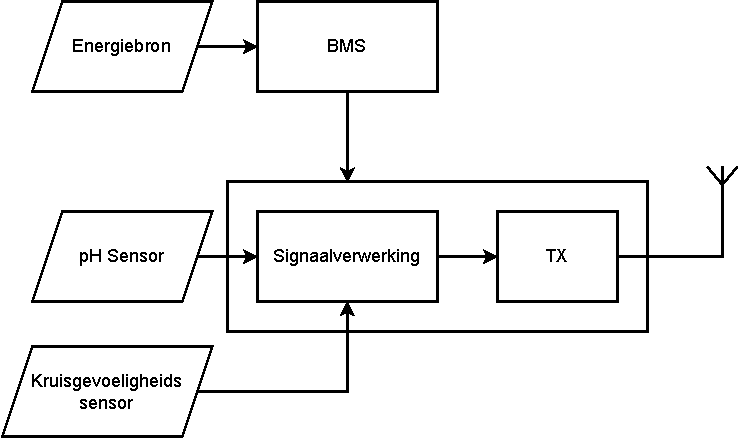
\includegraphics[width=\textwidth]{img/system.pdf}
        \end{figure}
            
    \end{frame}
        
    
    % \end{frame}
    \subsection*{decompositie}
    \begin{frame}
        \frametitle{Functionele decompositie}
        \begin{figure}
            \centering
            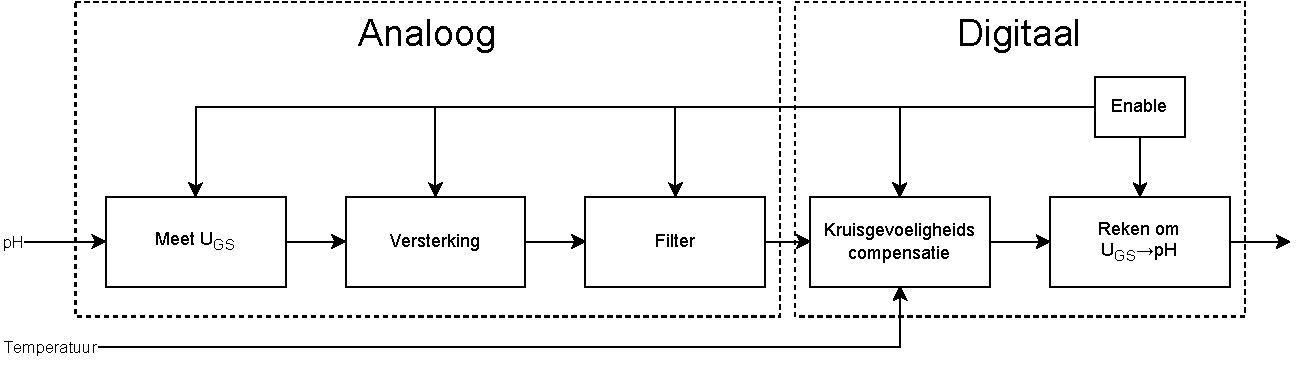
\includegraphics[width=\textwidth]{img/decompSignal.pdf}
        \end{figure}
        \begin{figure}
            \centering
            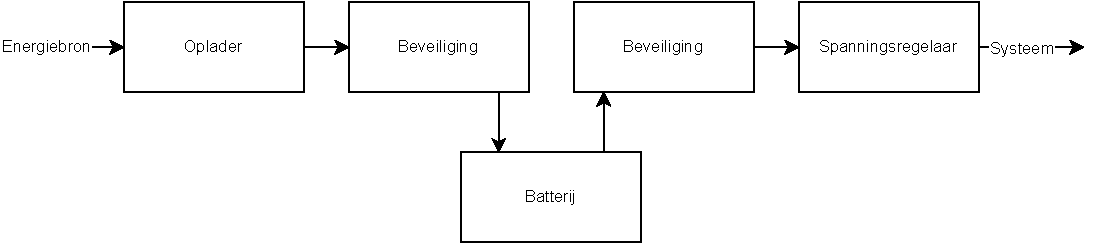
\includegraphics[width=\textwidth]{img/funcdDecompEnergy.pdf}
        \end{figure}    
    \end{frame}
    \subsection*{Energie \& ruis}
    \begin{frame}
        \frametitle{Energie \& ruisbudget verdelen}
    
        
    
    \end{frame}